% vim: set spell spelllang=es syntax=tex :

\section{OpenMP: Open Multi-Prossesing}

\emph{OpenMP} es una API de bibliotecas y directivas al compilador para la
definición de paralelismo de alto nivel para sistemas de memoria compartida en
\emph{C}, \emph{C++} y \emph{Fortran}\cite{ompWeb}. La ventaja de \emph{OpenMP}
es que permite la creación de regiones paralelas, secciones criticas, tareas y
puntos de sincronización, simplemente marcando un bloque de código con unas
pocas directivas al compilador. \emph{OpenMP} originalmente implementaba solo el
modelo de \emph{fork and join}, pero a partir de la versión $3.0$ se agrego el
modelo de tareas explicitas\cite{openmp08}. Ambos modelos fueron utilizados para
la implementación del sistema.

El modelo de \emph{fork and join} fue propuesto por primera ves en
\cite{conway1963}. En este modelo, la ejecución del programa se ejecuta con un
solo hilo al comienzo de se ejecución y durante sus secciones secuenciales, al
hilo inicial se lo llama hilo principal. Cuando se encuentra una región de
trabajo compartido (o \emph{worksharing region}) de $N$ tareas, el hilo
principal crea $N-1$ nuevos hilos. Cada hilo (incluido el hilo principal)
ejecuta una de las $N$ tareas. Esta etapa es llamada \emph{fork}. El hilo
principal no continua la ejecución secuencial hasta que no han finalizado todas
las tareas paralelas. A esta sincronización se la llama \emph{join}. La figura
\ref{conway} muestra un ejemplo en el cual se crean dos tareas paralelas. El
modelo de \emph{fork and join} puede aplicarse tanto para paralelismo de tareas
como de datos. 

\begin{figure}[!h]

	\centering

	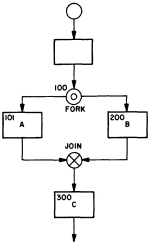
\includegraphics[width=0.25\textheight]{img/conway.pdf}

	\caption{Descripción original del modelo de \emph{fork and join}
	presentado por Melvin Conway en 1963\cite{conway1963}.}

	\label{conway}

\end{figure}

Dado que la creación de hilos suele ser una operación costosa, la mayoría de las
implementaciones de \emph{OpenMP} suelen no destruir los hilos creados durante
el \emph{fork}, sino que se mantienen inactivos para ser reutilizados cuando se
encuentre otra región de trabajo compartido.

El segundo modelo implementado en \emph{OpenMP} a partir de la versión $3.0$ es
el de tareas. En este modelo cuando se encuentra una región de trabajo
compartido, se crea un conjunto de $N$ hilos de ejecución pero no se crean
tareas para esos hilos inmediatamente. Durante le ejecución de la región de
trabajo compartido, se crean tareas que son colocadas en una cola de ejecución.
Cuando un hilo de ejecución del conjunto esta libre se le asigna una tarea de la
cola de ejecución. Cuando un hilo termina de ejecutar una tarea, toma otra de la
cola de tareas o espera. Solo se destruyen los hilos cuando se termina la
ejecución de todas las tareas y se sale de la región de trabajo compartido.

Dado que la creación de las tareas se puede hacer luego de la creación de los
hilos de ejecución, este modelo permite una mayor distribución temporal de las
tareas creadas en una región compartida. También permite que una tarea cree
nuevas tareas dentro de la misma región.

\subsubsection{Directivas de OpenMP}

Para la creación de una región de trabajo compartido bajo el modelo de tareas se
utiliza la directiva \emph{omp parallel}, y para creación de las tareas dentro
de la región se utiliza la directiva \emph{omp task}.

En el caso de \emph{OpenMP}, su uso para paralelismo de datos se realiza
comúnmente a través de la directiva \emph{parallel for}, mientras que la
directivas \emph{parallel sections} y \emph{parallel section} son utilizadas
para el paralelismo de tareas.
